%!TEX root = ../main.tex
%=========================================================

\section{Introduction}

\er{changes:
\begin{itemize}
  \item mention there is a DHT but do not say it is Kademlia (in the background mention that it is inspired by Kademlia)
  \item DHT is not used as-is as a key value store (with a single location for a value) -- change the discussion on this as well (when saying we don't want centralization)
  \item the registration is done at randomly selected subsets of fixed number of nodes in increasingly-small subsets of peers, drawn from the DHT routing structure (buckets); the likelihood of finding 
\end{itemize}
}

Ethereum is one of \er{or \textbf{the} largest?} the largest decentralized platform currently in operation. \er{see the official numbers, 27.000 nodes in total? Source?}
While is is widely known for supporting the blockchain of the same name (also known as the \emph{mainnet}), the Ethereum platform is also home to a number of additional decentralized applications.
This includes blockchains used for test purposes (testnets such as \emph{Ropsted} or \emph{Rinkeby}), divergent blockchains resulting from a past fork (\emph{Ethereum classic}), alternative cryptocurrencies (\emph{Pirl}, \emph{Musicoin}), content delivery networks (\emph{Swarm}), or messaging applications (\emph{Whisper}). \er{maybe give more/more diversified examples? IPFS? Others? Why isn't IPFS on the plot btw?}
In 2018, a study of the Ethereum ecosystem~\cite{kim2018measuring} indicated that the platform featured no less than 4,076 such applications, and that this number will keep growing in the future. \er{this really reads as if the paper was written in 2018, don't we have more recent numbers? Ideally we would like to have them for several years and show the trend.}

\begin{figure}[t]
    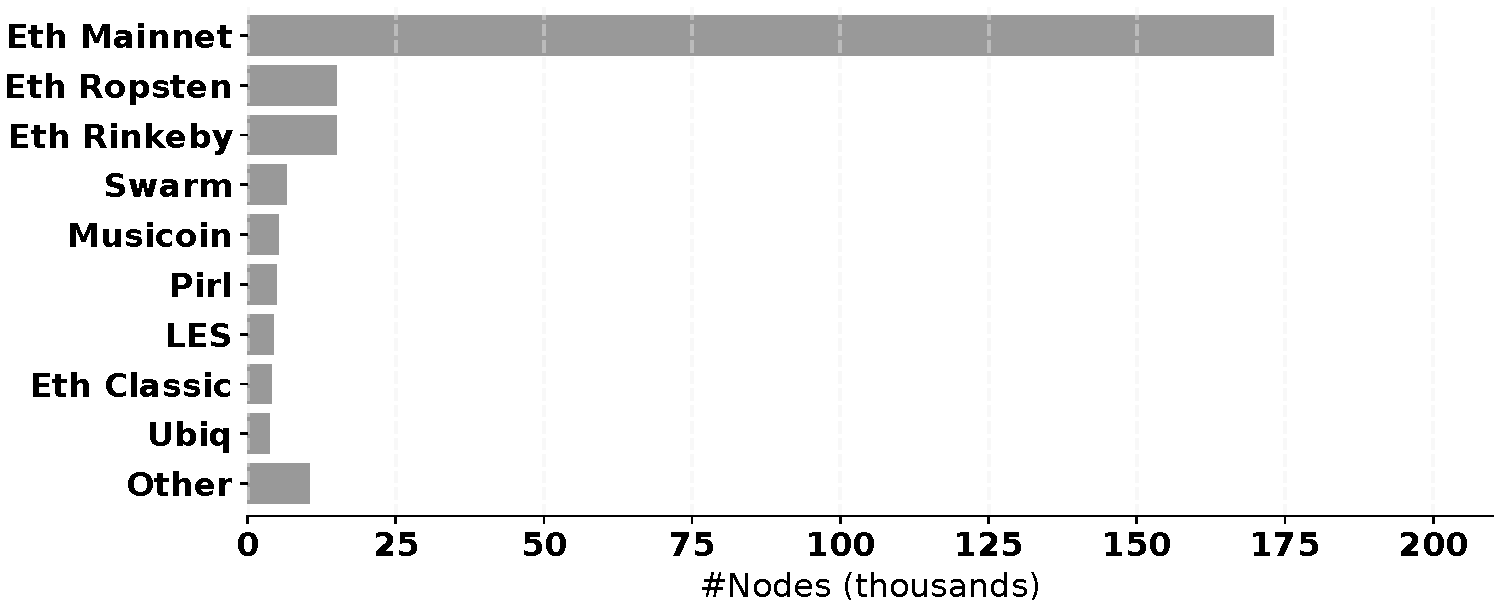
\includegraphics[width=1\linewidth]{img/ecosystem}
    % \vspace{-2mm}
    \caption{Number of different nodes identities witnessed in Ethereum's main applications, over an observation period of one year \protect\er{was it one year exactly?} (numbers reported by Kim et al.~\cite{kim2018measuring}).
    \protect\er{maybe give the date when the snapshot was taken. Also, ``Other'' should be ``Others''. We can also consider using a split x axis in order to avoid the very small lines for everything else than the mainnet. The figure is also not giving a sense of the long tail with networks of a few hundreds/thousands of nodes (our focus)}
    \protect\er{present relative numbers rather than absolute ones}
    % \vspace{-2mm}
    }
    \label{fig:ecosystem}
\end{figure}

Every node in the Ethereum platform participates to a \emph{global} peer-to-peer (P2P) network operating a distributed hash table (DHT)~\cite{maymounkov2002kademlia}. \er{how many nodes in this global network?}
% This global DHT is primarily used for periodic node discovery. % and not as a key-value store (i.e., lookup operations are never used).
The initial entry in the DHT leverages \emph{bootstrap nodes} operated by the Ethereum foundation, that provide a set of initial contact points, but subsequent maintenance of each nodes' view rely on periodic collection of random peers through DHT lookups.

In addition to joining the global network, every node must connect to one \emph{sub-network} formed of peers participating to its application of interest.
The size of these sub-networks can vary significantly.
\Cref{fig:ecosystem} depicts the size distribution of Ethereum's main applications.
This distribution features a \emph{long tail}, with a vast majority of applications formed of a few thousand nodes or less, much less than the mainnet or even than the testnets. \er{would be useful to give more precise quantiles, e.g., 80\% have less than 1.000 nodes, 90\% less than 200 nodes, etc.}

% Every node in the Ethereum platform participates to a \emph{global} peer-to-peer (P2P) network operating the Kademlia distributed hash table (DHT)~\cite{maymounkov2002kademlia}. \er{how many nodes in this global network?}
% Bootstrapping membership to this general network is handled by a number of trusted \emph{bootstrap nodes} operated by the Ethereum foundation, who provide an initial list of contact peers to nodes entering the network.
% Once joined, every node must connect to one or more sub-network(s) formed of peers participating to its application(s) of interest.
% The size of these sub-networks can vary significantly.
% \Cref{fig:ecosystem} depicts the size distribution of the platform main applications.
% This distribution features a \emph{long tail}, with a vast majority of applications formed of a few thousand nodes or less, much less than the mainnet or even than the testnets. \er{would be useful to give more precise quantiles, e.g., 80\% have less than 1.000 nodes, 90\% less than 200 nodes, etc.}

In this paper, we focus on the \emph{service discovery} mechanism, by which a node participating to the global P2P network discovers an application sub-network.
This mechanism returns a set of peers that are used as entry points to the P2P overlay specific to that application, as illustrated by \Cref{fig:subnetwork}.

\begin{figure}[b!]
    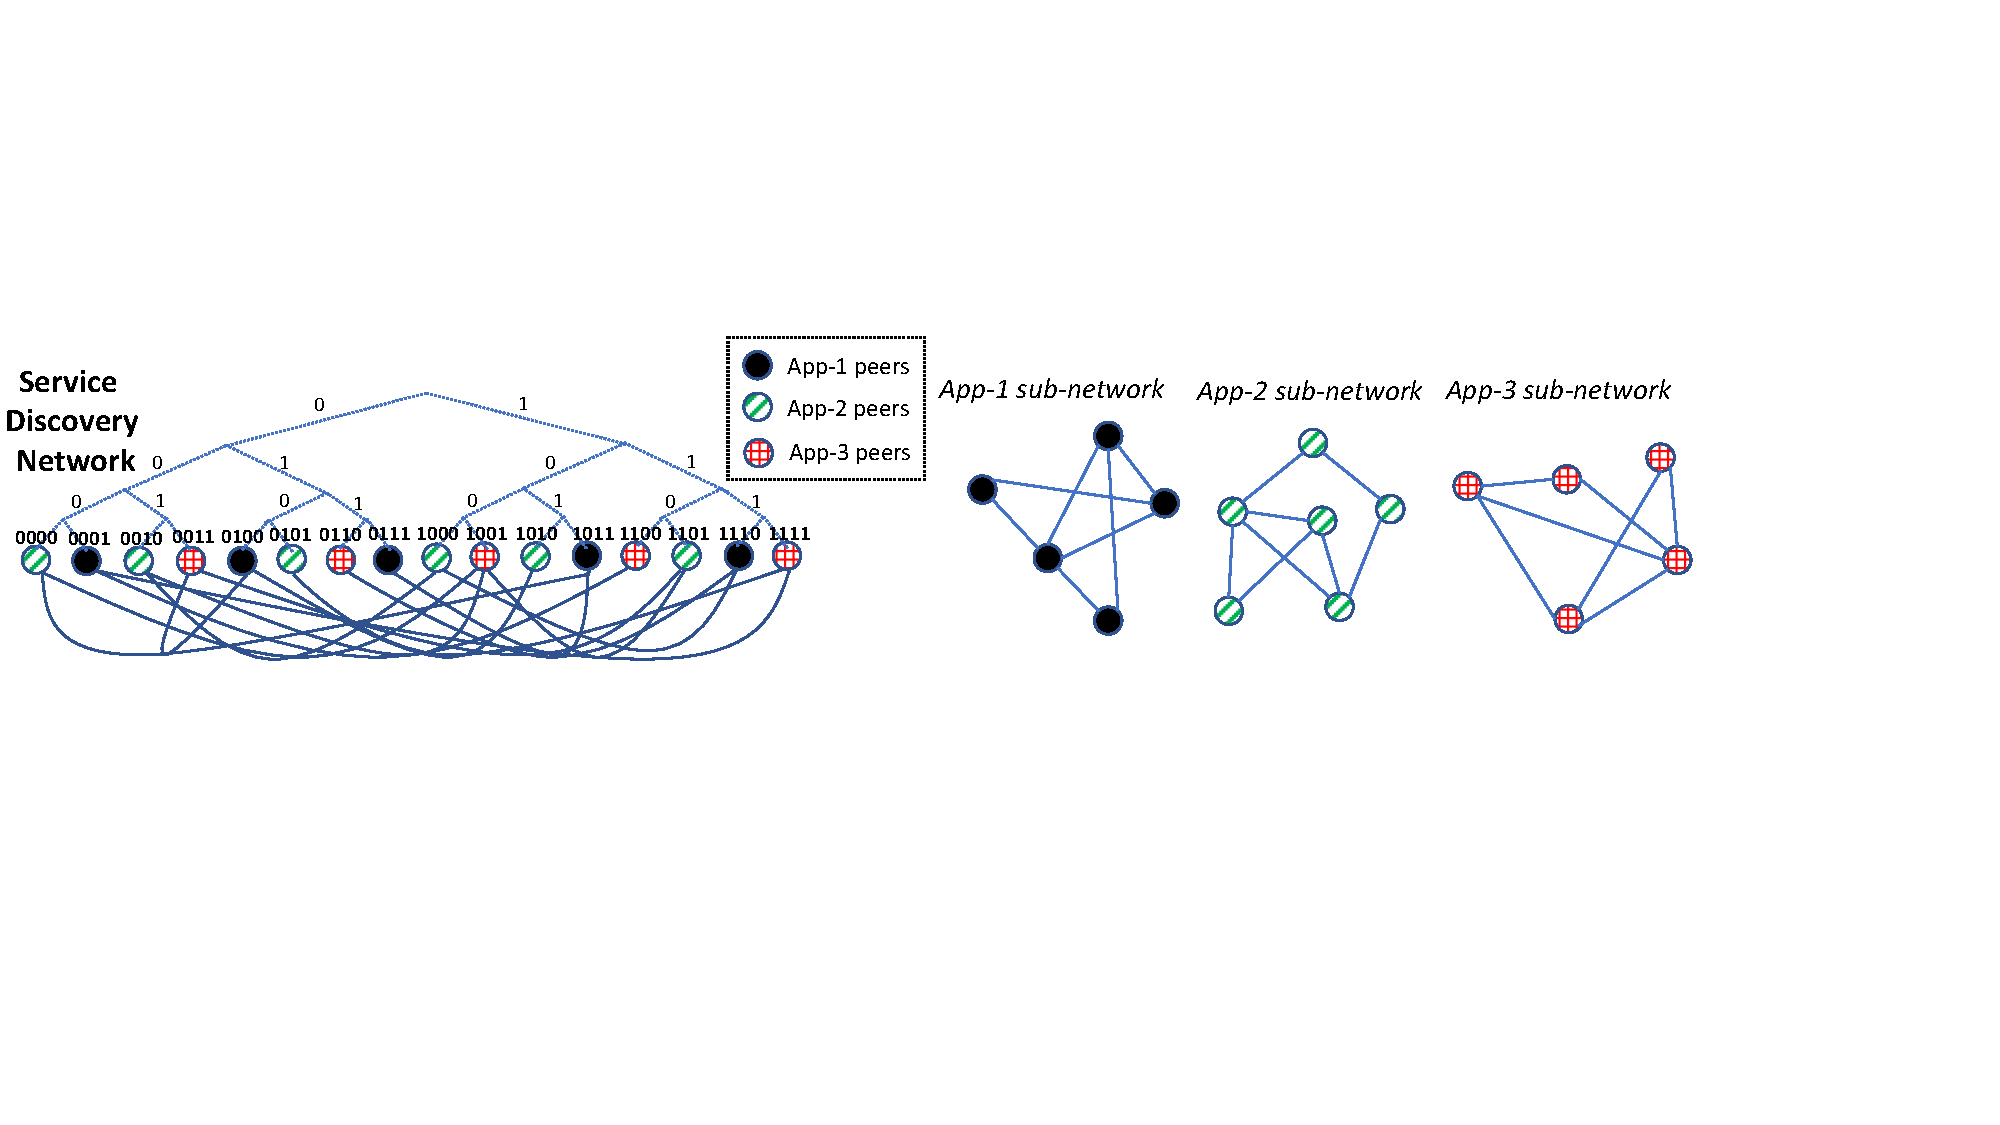
\includegraphics[width=1\linewidth]{img/subnetwork}
    \caption{Formation of application-specific sub-networks using a universal service discovery network.
    \protect\er{would be good to use different structures for the sub-networks, here they look quite similar}
    }
    \label{fig:subnetwork}
\end{figure}

Service discovery is a particularly sensitive mechanism in the Ethereum platform.
Its implementation must ensure that malicious participants to this open network are unable to bias its execution against a victim node or sub-network--and that, despite the ability of these adversaries to operate multiple Sybil identities.
Of particular importance is the protection against \emph{eclipse} attacks, where an adversary would lure its victim(s) into a sub-network formed of only nodes under its control. %, i.e., by returning only such nodes to a service discovery request.
Similarly, an adversary could wish to run \emph{denial-of-service} attacks against a specific application, preventing other nodes from discovering peers from the associated sub-network.
On the other hand, the mechanism must remain efficient and scalable.
It is not desirable, in particular, that it relies solely on a set of dedicated registry nodes maintaining the membership of each application, both for scalability and robustness reasons: Registry nodes for popular applications would quickly become overwhelmed, and attackers would have efficient strategies to place Sybils on the path to registry nodes, or act as such nodes themselves.
% \er{also the applications may want to hide themselves (but this clashes completely with our announcement approach)}

The current service discovery mechanism used in the Ethereum platform is part of discv4, a set of protocols leveraging the global DHT.
It employs a simple but robust \emph{random walk} approach.
A node willing to join an application's sub network simply contacts individually a series of nodes collected from random lookups on the DHT, repeatedly checking application membership until it has collected enough peers. % to join the sub-network.
This approach offers good resilience to malicious behaviors
% , and in particular against denial-of-service attacks, 
but it suffers from very poor scalability and performance, in particular for small sub-networks.
% While using the Kademlia DHT as a key/value store to maintain membership information at a specific node or replica group would allow deterministic lookup of this information, regardless of the application's popularity, this solution would suffer from very poor robustness to attacks and would lead to hotspots and overload for nodes in charge of popular services.

\smallskip
\noindent
\textbf{Contributions.}
%
We detail in this paper \sysname, a novel service discovery mechanism for large-scale, decentralized platforms and its application to Ethereum.
\sysname targets a balance between robustness, i.e., the ability to resist malicious behaviors and Sybil identities, and efficiency, i.e., fast service discovery even for small applications and good load-balance over participating nodes.
\sysname is integrated into the upcoming version of Ethereum, as part of the replacement of discv4 mechanisms ... \er{provide details here already. Why don't we call it discv5 anymore?}

After providing background knowledge and reviewing the current service discovery mechanism of Ethereum in \Cref{sec:background}, we detail \sysname as follows.

In \Cref{sec:placement}, we present how this new protocol enables nodes, members of application sub-networks, to \emph{advertise} their membership to these applications in the form of \emph{service advertisements}.
Any node can act as a \emph{registrar} and store advertisements for any topic.
In contrast with a direct use of the DHT as a key-value store, however, in \sysname service advertisements propagate to a pseudo-random subset of all nodes in the global network.
The density of advertisements for an application increases as a DHT lookup approaches its associated key in the DHT overlay structure.
% As such, \sysname enables efficient lookup of advertisements for any given service.

Robustness, load balancing, and efficiency for the discovery of smaller sub-networks all rely on a novel \emph{admission protocol}, by which registrars accept or reject incoming service advertisements.
This mechanism is detailed in \Cref{sec:registration}.
It ensures that advertisers cannot flood advertisements at a registrar even when deviating from the protocol or operating Sybils, and that less popular topics get sufficiently high probability to be represented and looked up. \er{not sure about this sentence, we do not provide any bound, this is all probabilistic.} \er{I did not keep the comment about the intermediary state as I am not sure what it is about.}

At the core our novel admission protocol lies the need for registrants to respect a waiting time imposed by the registrars before being able to successfully register their advertisement.
We discuss the design and dynamics of the waiting function in \Cref{sec:waitingTime}.
We design a function that allows limiting the amount of resources used by each node, promotes diversity of topic advertisements stored by each node, and protects against a vast range of malicious behaviors.

We implemented \sysname in a simulator as well as in the code base of the upcoming version of Ethereum.
We intend to release the full code and dataset of our experiment open source with the unblinded version of this paper.
Our results show ...

